\chapter{Implémentation}
\label{ch:impl}

%TODO ajouter problèmes rencontrés ou intégrer ailleurs et parler de la sérialisation et du problème de connexion socket que j'ai eu, voir si autres problèmes
\section{Choix d'implémentations}
\subsection{Langage}
Au départ le choix du langage s'est porté sur sagemath (framework python) afin de mieux comprendre les différents calculs et faire un premier POC du chiffrement/déchiffrement.
Cependant l'implémentation du POC était lente et le changement d'algorithme pour les pairings était difficile.
Je me suis donc orienté sur le C pour avoir de meilleures performances et pouvoir mieux gérer la mémoire de mon implémentation. Pour pouvoir faire facilement des calculs sur les courbes elliptiques et les pairings en C il me fallait une librairie ce que je décris dans la section suivante. Comme on peut le voir sur la table \ref{table:comparisonTimeAlgo}, une différence des temps d'exécution entres les deux langages. Il faut cependant mettre en lumière que les temps sont calculés avec des courbes différentes et des couplages différents (Sage avec des Weil pairings, C avec ate pairings).

\begin{table}[h!]
	\centering
	\begin{tabular}{ |p{3cm}||p{3cm}|p{3cm}| }
		\hline
		\multicolumn{3}{|c|}{Temps des algorithmes entres langages [s]} \\
		\hline
		Algorithms& C &Sage\\
		\hline
		Setup   & 0.2856898 & 6.5858234\\
		Encrypt & 0.0061584 & 7.6450206\\
		Decrypt & 0.00951 & 3.3274426\\
		\hline
	\end{tabular}
\caption{Table de comparaison des temps d'exécution pour les différents algorithmes de Certificateless Cryptography }
\label{table:comparisonTimeAlgo}
\end{table}

\subsection{Librairie cryptographique}
%TODO + d'explications sur les librairies et les choix faits (retrouver l'endoit où l'on dit que RELIC est plus efficient et est plus fait pour les POCs etc)
La librairie utilisée est RELIC Toolkit~\cite{relic-toolkit}, c'est une librairie en cours de développement qui se veut efficiente. Sa concurrence avec MIRACL m'a fait hésiter dans mon choix, mais MIRACL est plus codée en~ C++ avec des équivalences en C j'ai donc choisi RELIC. De plus j'ai trouvé par exemple que RELIC était généralement plus adapté dans le domaine universitaire pour des POC puis il est plus efficient que d'autres librairies~\cite{performanceRELIC}.
\subsection{Courbe utilisée}
La courbe utilisée pour le POC est la BLS12-P381, en effet cette courbe est assez efficiente et compatible avec les pairings. De plus RELIC l'a dans ses options et fonctionne bien, elle a un niveau de sécurité de 128bits. Je voulais prendre une courbe avec une plus grande sécurité cependant RELIC ne l'a pas encore totalement implémenté (certains tests concernant $\mathbb{G}_2$ ne passes pas), mais la librairie étant toujours en cours de développement il faudrait suivre ça de près, le code ne changerait en effet pas.
% TODO voir si KDF n'st pas mieux ? ou même générique de libsodium
\subsection{Dérivation de la clé AES}
Le but de mon schéma certificateless est de chiffrer puis signer une clé AES qui permettra à mon message d'avoir un chiffrement authentifié. Pour cela il me faut dériver un élément de $\mathbb{G}_t$ en clé AES, en effet le chiffrement dans le schéma certificateless se fait sur un élément de $\mathbb{G}_t$.\\
Pour cela j'ai utilisé une fonction permettant d'écrire sous forme compressée cet élément en bytes (fourni par la librairie RELIC utilisé et la fonction gt\_write\_bin()). Puis j'ai effectué un hachage avec SHA256 dessus, ainsi le résultat du hachage est une clé de 256 bits utilisable par AES-256-GCM. La fonction de hachage doit être par conséquent cryptographiquement sûre.
\subsection{Fonctions de hachage - signature}
Pour le schéma de signature il nous faut plusieurs fonctions de hachage différentes, en effet ce schéma est basé sur le \textit{Random Oracle Model} comme définit dans le chapitre \ref{ch:analysis}. Pour appliquer cela j'ai utilisé la même méthode de mapping disponible ans RELIC pour mapper une char array (tableau de byte) à un point sur G2 à savoir g2\_map.
Pour H1, la première fonction de hachage j'ai simplement utilisé cette fonction directement, mais pour H2 et H3 j'ai ajouté un byte devant les données à mapper respectivement les bytes '01' et '02'. Ceci afin de séparer les domaines des résultats des hashs, cela s'appelle du \textit{Hash Domain Separation}. En effet l'on peut voir dans ce draft~\cite{irtf-cfrg-hash-to-curve} définit comme une simulation pour prendre en compte plusieurs \textit{Random Oracle}.
\subsection{Sérialisation des données}
Pour la sérialisation des données, typiquement les clés publiques et les clés privées partielles envoyées en réseau ou les clés publiques enregistrées dans les fichiers par exemple, j'ai utilisé la librairie binn\footnote{\url{https://github.com/liteserver/binn}}. Cela permet de packer facilement des données binaires, pour cela RELIC met à disposition des méthodes g1\_write\_bin g1\_read\_bin qui a permis de faire ces enregistrements binaires. Ainsi les transferts de données sont simplifiés. Cependant il faut faire attention à certaines choses, on ne peut lire et écrire simultanément à l'aide de binn, si l'on crée un objet via un buffer on ne pourra modifier cet objet. Cela m'a posé des problèmes pour l'enregistrement des données secrètes, j'ai donc du copier l'objet lu pour pouvoir le modifier et sauver les nouveau paramètres.
\subsection{Enregistrement des clés publiques (serveur)}
Pour l'enregistrement j'ai utilisé une petite base de données NoSQL stockant les clés publiques des utilisateurs sur le KGC. Cela permet de facilement récupérer une clé publique pour un utilisateur si besoin. Pour implémenter cela j'ai utilisé la librairie UnQlite\footnote{\url{https://unqlite.org/}}. J'ai stocké les clés publiques pour le schéma de signature et de chiffrement séparément, en effet, l'entrée pour la signature porte le nom "signature/ID" et le chiffrement "encryption/ID".
\section{Implémentation clés  de chiffrement}
Pour pouvoir implémenter ce schéma de chiffrement et signature certificateless dans un système hybride il a fallu penser à une manière d'encapsuler la clé et les données. Pour cela j'ai essayé de faire un système comparable à la figure \ref{fig:encapsulate}. 
\begin{figure}[h!]
	\centering
	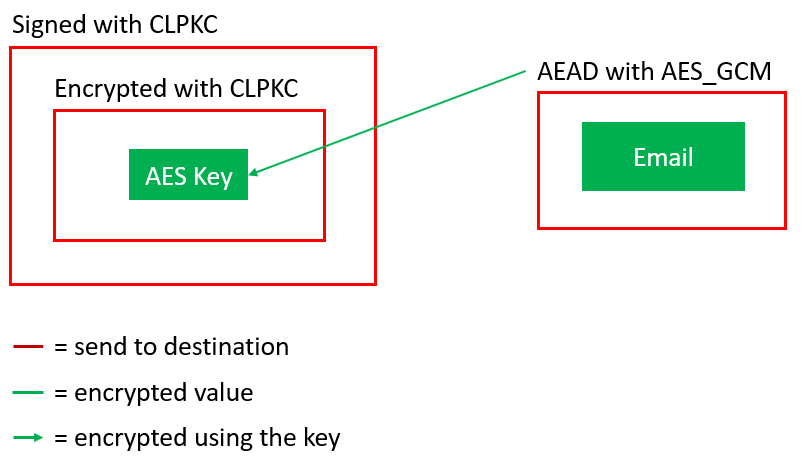
\includegraphics[width=12cm]{images/schemaEncapsulation.png}
	\caption{Schéma encapsulation des données}
	\label{fig:encapsulate}
\end{figure}

\section{Fonctionnement global POC (KGC)}
Ici je présente le fonctionnement global de mon implémentation du KGC pour mon POC. De plus je présente les problèmes connus et des propositions d'améliorations.
\subsection{Fonctionnement}
Le KGC est un élément important du protocole, en effet c'est lui qui va fournir une partie de la clé privée de l'utilisateur. De plus dans mon cas il permet de distribuer les clés publiques de ses utilisateurs, mais habituellement on fera plutôt appel à un serveur dédié pour la gestion des clés.\\
Par mesure de généricité j'ai établi des codes d'opérations (arbitraires) afin de définir les opérations demandées au serveur par le client. Cela à l'aide de la librairie binn et les constructions d'objets proposés.\\
\paragraph*{Structure des paquets reçus.}
Pour la structure des paquets que le KGC va traiter ils se présentent sous la forme d'un objet binn qui a comme propriétés au moins un code d'opération \textbf{opCode} et un \textbf{ID} associé. Cela permet de trier le paquet et de l'associer à une opération afin de traiter la donnée amenée avec le paquet. L'ID sert aussi différemment en fonction des codes employés.\\
Ainsi un paquet typique sera : \\
\{opCode: PK, ID : alice@wonderland.com, payload : xxx\}
\paragraph*{Codes d'opérations.}
Les différents codes d'opérations sont :
\begin{itemize}
	\item HELO : Permet de s'annoncer au KGC pour la première fois, le KGC répondra systématiquement avec les paramètres globaux du système. Cela implique la Master Public Key de chiffrement du KGC ainsi que celle du schéma de signature. 
	\item PK : Permet d'annoncer les clés publiques de l'utilisateur avec un certain ID. Le paquet est composé de \{ID : alice@wonderland.com, opCode : PK, PKE : base64 de la PKE, PKS : base64 de la PKS\}. La PKE est encodée en base64 par le client est envoyée au serveur. Elle est aussi représentée à l'aide d'un objet binn mais le serveur n'a pas besoin d'en prendre connaissance, il l'a stocke donc tel quel dans la base de donnée NoSQL. La même chose est faite pour la PKS, la clé publique pour la signature.
	\item GPE : Permet de récupérer la clé publique de chiffrement (utile pour chiffrer un message) d'un utilisateur ayant l'ID mentionné. Ainsi le serveur va simplement regarder dans la base de donnée pour "encryption/ID" et récupérer la clé encodée en base64 et la renvoyer à l'utilisateur. Si le serveur ne trouve pas cette clé il va renvoyer une erreur dans l'objet et ainsi à la réception on va d'abord regarder cette erreur.
	\item GPS : Fonctionne de la même manière que "GPE" mais pour les clés publiques de Signature (utile pour vérifier une signature).
	\item SE : Permet de faire la "Signature Extraction" et donc de demander la Partial Private Key pour l'utilisateur ID. Utilisé lors de la signature d'un message afin de construire sa clé privée et de signer le message avec. 
	\item EE : Permet de faire la "Encryption Extraction" et donc de demander la Partial Private Key pour l'utilisateur ID. Utilisé lors du déchiffrement d'un message pour reconstruire sa clé privée.
\end{itemize}
\subsection{Problèmes connus}
\subsection{Améliorations}
Quelques améliorations qui seraient possibles mais dont j'ai pas eu le temps de m'occuper :
\paragraph*{Vérification email.}
Implémentation d'une vérification par email afin d'être sûr que l'adresse email annoncée appartient bien à l'utilisateur qui s'authentifies pour la première fois. Typiquement lors du "HELO", l'on pourrait envoyer un mail de vérification avec un code sur l'email annoncé (s'il n'est pas dans la base de données) et demander le code envoyé avant de pouvoir uploader sa clé publique. Ainsi le client devrait pouvoir implémenter cette fonctionnalité aussi. Cela permettrait d'être sûr que tel utilisateur a effectivement tel email.
% TODO : voir avec Alex si garder ou non
\paragraph*{Zero-Knowledge proof pour PPK.}
On a vu dans les modèles d'adversaires définit par Al-Riyami et Paterson~\cite{DBLP:conf/asiacrypt/Al-RiyamiP03} qu'un adversaire pourrait obtenir les PPK des utilisateurs et ne pas réussir à déchiffrer des messages. Mais avec du Zero Knowledge l'on pourrait ajouter une sécurité supplémentaire pour ne pas délivrer à n'importe qui des PPK.
\section{Fonctionnement global POC (Client)}
Ici je présente le fonctionnement global de l'implémentation du client mail sécurisé pour mon POC, des améliorations possibles et des problèmes connus.
\subsection{Fonctionnement}
Je vais dépeindre le fonctionnement de mon POC ici et les différentes fonctionnalités que j'ai implémentée au client de mon POC.
\paragraph*{Sécurité connexion mail.}
Pour la connexion au serveur SMTP / IMAP j'ai fait attention à la connexion sécurisée pour éviter de \textit{leak} des mots de passe des utilisateurs du POC. En effet, cela permet de chiffrer les communications avec les serveurs de Gmail.
\begin{figure}[h!]
	\centering
	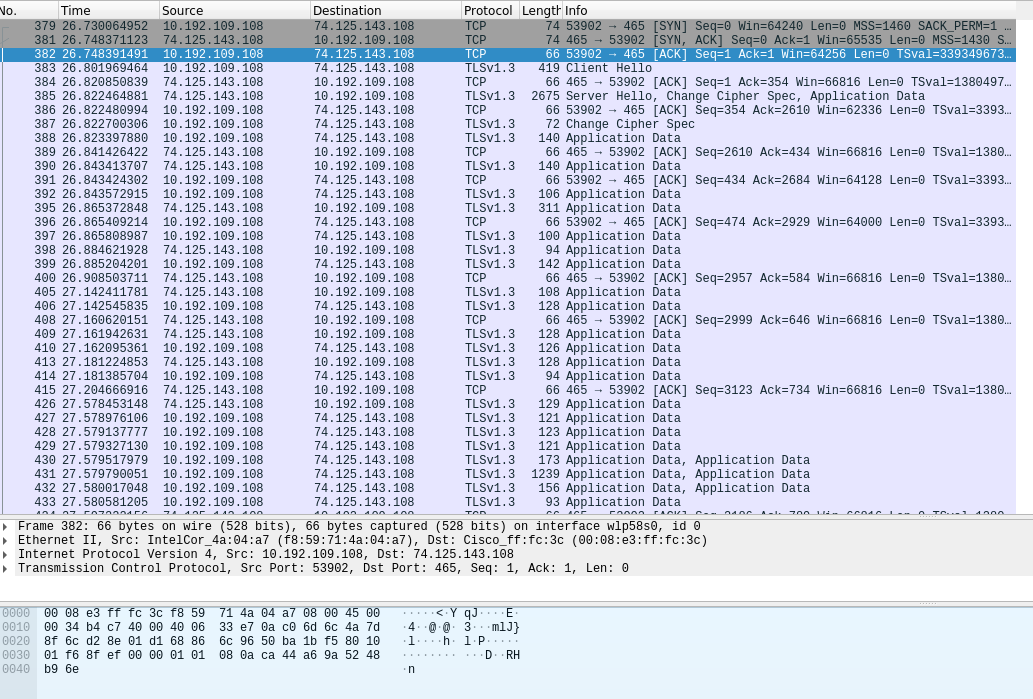
\includegraphics[width=14cm]{images/packetProofEncrypted.png}
	\caption{Connexion SSL/TLS avec le serveur email}
	\label{fig:securityProofEmail}
\end{figure}
%TODO : présenter des captures de paquets chiffrées de connexion IMAP et SMTP
\subsection{Problèmes connus}
Les problèmes qu'il reste à résoudre à ce jour :
\paragraph*{Développement sécurisé.}
ors du développement j'ai fait attention au maximum d'avoir le moins possible de fuite mémoires à l'aide de sanitizers et de valgrind. Cependant cela ne suffirait pas pour une application correctement sécurisée, il faudrait mettre à 0 les structures utilisées et qui stockent des informations confidentielles.
\subsection{Améliorations}
Les améliorations à amener dans le client :
\paragraph*{Multiples destinataires.}
Pour le moment l'implémentation ne prends pas en compte une situation où un mail doit être envoyé à des destinataires multiples, c'est une fonctionnalité importante à mettre en œuvre dans une implémentation de client mail. Pour ce faire il faudra spécifier dans les headers l'utilisateur ciblé par tel cipher et signature. Ainsi lors de la réception le client prendra les options X-ID-CIPHER-B64 p.ex. Ou alors trouver un moyen d'envoyer un mail différent à chaque utilisateur, sans perdre la possibilité qu'un destinataire puisses choisir de répondre à tous.
\paragraph*{Possibilité d'ajouter des pièces jointes.}
Pour le moment la possibilité d'ajout de pièces jointes n'a pas été pris en considération. Cependant une des librairies choisies pour la réception des emails pourrait composer des messages contenant des pièces jointes. Il faudrait ainsi les chiffrer avec la clé symétrique avant de l'ajouter dans le mail.
\paragraph*{GUI.}
Mettre ne place une interface utilisateur pour le client mail, cela aiderait à rendre le chiffrement plus transparent et plus simple pour l'utilisateur. En effet demander à l'utilisateur d'écrire son mail au terminal n'est pas spécialement agréable.
\section{Comparaisons avec état de l'art}
Dans cette section je vais présenter les différents protocoles et implémentations existantes présentées au chapitre \ref{ch:analysis} et les comparer à mon implémentation. Tout d'abord en présentant les différentes propriétés cryptographiques puis les temps d'exécution.

% TODO à analyser et remplir correctement
\subsection{Propriétés cryptographiques}
Ici je fais un comparatif sur les différentes propriétés cryptographiques que les systèmes de mails sécurisés proposent avec mon implémentation Certificateless. On peut le voir dans la table \ref{table:comparisonProperties}.
\begin{table}[h!]
	\centering
	\begin{tabular}{ |p{3cm}||p{3cm}|p{3cm}| }
		\hline
		\multicolumn{3}{|c|}{Comparaisons des propriétés cryptographiques proposées} \\
		\hline
		Implémentations & E2EE & Forward Secrecy\\
		\hline
		CLPKC-POC   & Oui & Oui\\
		PGP & Oui & Non\\
		S/MIME & Oui & Non\\
		\hline
	\end{tabular}
	\caption{Table de comparaison des différentes propriétés cryptographiques }
	\label{table:comparisonProperties}
\end{table}
% TODO si le temps le permet faire des calculs sur les temps de chiffrement / déchiffrement
\subsection{Temps des différentes implémentations}
Comparasion du temps mis pour chiffrer et signer / déchiffrer et vérifier un mail entres les différentes implémentations existantes. Dans la table \ref{table:comparisonTime} l'on voit les calculs faits.
\begin{table}[h!]
	\centering
	\begin{tabular}{ |p{3cm}||p{3cm}|p{3cm}| }
		\hline
		\multicolumn{3}{|c|}{Comparaisons des temps d'exécution entres différentes implémentations proposées} \\
		\hline
		Implémentations & Chiffrement & Déchiffrement\\
		\hline
		CLPKC-POC   & 0.0061584s & 0.00951s\\
		PGP & 0 & 0\\
		S/MIME & 0 & 0\\
		\hline
	\end{tabular}
	\caption{Table de comparaison des temps d'exécution entres les implémentations de mails chiffrés}
	\label{table:comparisonTime}
\end{table}
\subsection{Overhead induit}
Ici je présente les différents \textit{overhead} que j'ai remarqué en utilisant les différents systèmes de mails sécurisés analysés au chapitre \ref{ch:analysis}. Dans le tableau \ref{table:comparisonOverhead} on voit la taille d'overhead induit par les différents systèmes testés.
\begin{table}[h!]
	\centering
	\begin{tabular}{ |p{3cm}||p{5cm}|p{6cm}| }
		\hline
		\multicolumn{3}{|c|}{Comparaisons de l'overhead induit dans un mail} \\
		\hline
		Implémentations & Taille overhead & Contenu\\
		\hline
		CLPKC-POC   & Environ 1200 bytes & Signature, timestamp, nonce, Encrypted Session Key\\
		PGP & Environ 300 bytes & Encrypted Session key\\
		S/MIME & 0 & TODO\\
		\hline
	\end{tabular}
	\caption{Table de comparaison des différents overhead en rapport avec les solutions existantes }
	\label{table:comparisonOverhead}
\end{table}